%%%%%%%%%%%%%%%%%%%%%%%%%%%%%%%%%%%%%%%%%%%%%%%%%%%%%%%%%%%%%%%%%%%%%%
% LaTeX Example: Project Report
%
% Source: http://www.howtotex.com
%
% Feel free to distribute this example, but please keep the referral
% to howtotex.com
% Date: March 2011 
% 
%%%%%%%%%%%%%%%%%%%%%%%%%%%%%%%%%%%%%%%%%%%%%%%%%%%%%%%%%%%%%%%%%%%%%%
% How to use writeLaTeX: 
%
% You edit the source code here on the left, and the preview on the
% right shows you the result within a few seconds.
%
% Bookmark this page and share the URL with your co-authors. They can
% edit at the same time!
%
% You can upload figures, bibliographies, custom classes and
% styles using the files menu.
%
% If you're new to LaTeX, the wikibook is a great place to start:
% http://en.wikibooks.org/wiki/LaTeX
%
%%%%%%%%%%%%%%%%%%%%%%%%%%%%%%%%%%%%%%%%%%%%%%%%%%%%%%%%%%%%%%%%%%%%%%
% Edit the title below to update the display in My Documents
%\title{Project Report}
%
%%% Preamble
\documentclass[paper=a4, fontsize=11pt]{scrartcl}
\usepackage[T1]{fontenc}
\usepackage{fourier}

\usepackage[english]{babel}			% English language/hyphenation
\usepackage[protrusion=true,expansion=true]{microtype}	
\usepackage{amsmath,amsfonts,amsthm}   % Math packages
\usepackage[pdftex]{graphicx}	
\usepackage{url}
\usepackage{lipsum}
\usepackage{listings}
\usepackage{color}
\usepackage{framed}
\usepackage{graphicx}
\usepackage{hyperref}

%%% Custom sectioning
\usepackage{sectsty}
\allsectionsfont{\centering \normalfont\scshape}
\usepackage[top=1in, bottom=0.75in, left=1in, right=1in,headsep=1cm]{geometry}

\newlength\tindent
\setlength{\tindent}{\parindent}
\setlength{\parindent}{0pt}
\renewcommand{\indent}{\hspace*{\tindent}}

%%% Custom headers/footers (fancyhdr package)
\usepackage{fancyhdr}
\pagestyle{fancyplain}
\fancyhead{}						% No page header
\fancyfoot[L]{}						% Empty 
\fancyfoot[C]{}						% Empty
\fancyfoot[C]{\thepage}				% Pagenumbering
\renewcommand{\headrulewidth}{0pt}	% Remove header underlines
\renewcommand{\footrulewidth}{0pt}		% Remove footer underlines
\setlength{\headheight}{13.6pt}


%%% Equation and float numbering
\numberwithin{equation}{section}		% Equationnumbering: section.eq#
\numberwithin{figure}{section}			% Figurenumbering: section.fig#
\numberwithin{table}{section}			% Tablenumbering: section.tab#


%%% Maketitle metadata
\newcommand{\horrule}[1]{\rule{\linewidth}{#1}} 	% Horizontal rule

\title{
	%\vspace{-1in} 	
	\usefont{OT1}{bch}{b}{n}
	\normalfont \normalsize \textsc{University of Texas at Austin\\IEEE Robotics and Automation Society} \\ [25pt]
	\horrule{0.5pt} \\[0.4cm]
	\huge Introduction to C Programming \\ 
		\vskip 0.1in
		\large Embedded System Level Design
	\horrule{2pt} \\[0.5cm]
}
\author{
	\normalfont 			\normalsize
        Kevin Gilbert\\[-3pt]		\normalsize
	21 October 2014
}
\date{}

%%% Begin document
\begin{document}
\maketitle
\section{Overview}
This document is intended to provide a crash course to embedded level specific C programming, and assumes you have no previous experience in software development. A brief overview of assembly, machine code, and instruction set architectures will be covered in the following sections to provide a basis for understanding the mechanics behind C. Dr. Patt's EE306 textbook covers C in later chapters as well if you want more additional information. This is a highly extensive subject that spans very deeply; as a result this paper won't be enough to provide you with a full background. I hope however that this is sufficient to have a baseline working understanding of the language. Subsequent courses will go much deeper into the subject, so you will be ahead of the curve if you began to gain an understanding at this stage already. 

\section{Toolsets}
The best way to learn programming is through experience.
\href{http://codepad.org}{Codepad} or \href{http://ideone.com/}{Ideone} can be used as online compilers to help learn the mechanics of C. The later sections will contain basic examples that I recommend you follow along  and play with. The last sections will cover embedded specific level programming converging with a focus on the TI LM4F launchpad in particular. Besides the online IDEs linked to above, development in a Linux environment is great for this. The GNU Compiler Collection (GCC) and the GNU Debugger (GDB) are great command line compiler and debuggers for C. Mac OS has access to these tools through the terminal as well with some additional work. Windows has much less native support for application based C development. Compilers like Eclipse and Microsoft Visual Studios work but are much bulkier. What is also often done is emulate gcc using tools such as MinGW. However, for most embedded platforms the code is compiled to the target platform's ISA and flashed onto the chip. Most producers will include IDEs to facilitate this, most notable examples being Keil or CodeComposer by TI for the launchpads, or the Arduino IDE. As stated, the largest difference between application level C development, and embedded system level C development is the target application's architecture. Application files are targeted towards the host OS. Think of generating an executable file. Embedded compilers will create output files for the embedded application specifically. For learning the mechanics of how to program in C, I will begin with more of an application approach so that the output can be more easily seen.\\

ECE students at UT Austin can get SSH access to Linux machines on campus through this \href{http://www.ece.utexas.edu/it/remote-Linux}{link}. The bottom of the page mentions Putty, a free ssh client for windows. If you want to learn some Linux, I recommend using this tool or creating a virtual machine and running a simple Linux distribution such as Ubuntu or Debian. Ubuntu is more user friendly and is typically the least jarring coming straight from a Windows environment, but comes with a lot of unnecessary components I find. Lubuntu or Xbuntu run the same core, but have a different and more lightweight Graphical User Interface (GUI). Debian is the slightly smaller and more stable version of Ubuntu. Arch Linux is absolutely bare bones and very lightweight, but has the highest learning curve. Feel free to experiment and try out different versions.

\section{Levels of Abstraction}
The first step I would like to take is to break the levels of abstraction for software to hardware development. Dr. Patt is a large proponent of this, and the following figure is taken from his course notes.
\vskip 0.1in
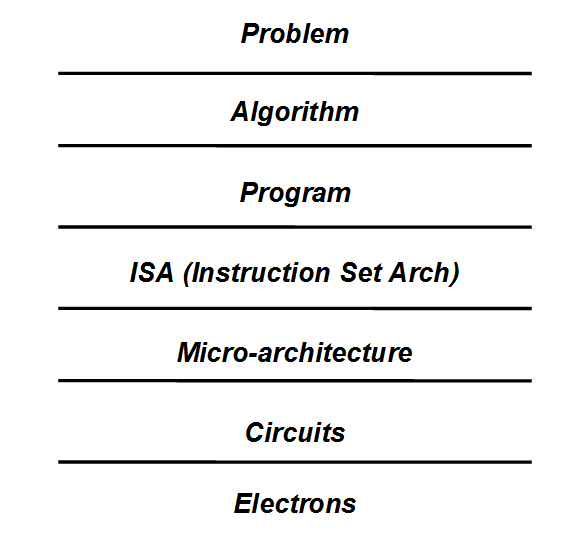
\includegraphics[width=\textwidth]{images/levels_of_abstraction}
\vskip 0.05in
\centerline{\textbf{Figure 1. }Levels of Software Abstraction - Dr. Patt}

\newpage
Understanding all of the above layers in full detail could be a complete course on its own, so rather than try to poorly explain everything with a glancing overview I will focus on the two middle sections: the Instruction Set Architecture (ISA) and the Program layers.

\subsection{Instruction Set Architectures}
For those of you currently taking Introduction to Computing (EE306), this concept will be more familiar to you. At the lowest level, a computer provides a way to control electrons. This is done through the application of potential energy (voltage) and current in the form of circuits. These circuits in turn are organized through the microarchitecture. This is where the software and hardware begin to merge and blur the lines between the two levels. The ISA comprises the set of opcodes implemented by the microarchitecture. An example would be what most computers run today. the x86 ISA makes up most desktop and laptop cores. However how x86 is implemented in hardware is ambiguous. The Intel i3, i5, and i7 for example are all x86 processors, but implement how the instructions are executed in different manners through the microarchitecture. \\

The reason I mention this is because it is fundamental to understanding the power C has, and why C in particular is used for embedded programming. In terms of abstractions, C is very close to the hardware and ISA. The C language maps very closely to assembly. The particular set of opcodes and registers used depends on the end application. When you compile a C file with GCC on your desktop running with an x86 processor, an x86 binary file is generated. When you compile your Robotathon code in Keil, an ARM binary file is generated. What I mean by binary files in this case is a file comprised of 1's and 0's. A computer operates in binary, which is obviously very difficult for humans to read. Assembly languages were created to make programming more human readable. A line of assembly gets translated into a binary string. For example the instruction to add two registers and store the results would be \\
\centerline{\textit{ADD R2, R1, R0}} \\
in an ARM machine. The opcode for ADD had a unique binary representation, as does each register field. This means that when the computer fetches this instruction to execute it, it receives a string of 1's and 0's uniquely identifiable as the above instruction. Below is an example of a simple C file being compiler into x86 assembly. The program allocates three integer variables (more on that later), assigns the first two values of 1 and 2, adds the two numbers and stores the result into the third variable. This value is then returned. The result can be seen in the image.

\begin{framed}
	\begin{lstlisting}[language=C++,
	                   directivestyle={\color{black}}
        	            emph={int,char,double,float,unsigned},
                	     emphstyle={\color{blue}}
                	    ]
	int main(void) {
		int a, b, c;
		a = 1;
		b = 2;
		c = a + b;
		return c;
	}	
	\end{lstlisting}
\end{framed}

\newpage

\fbox{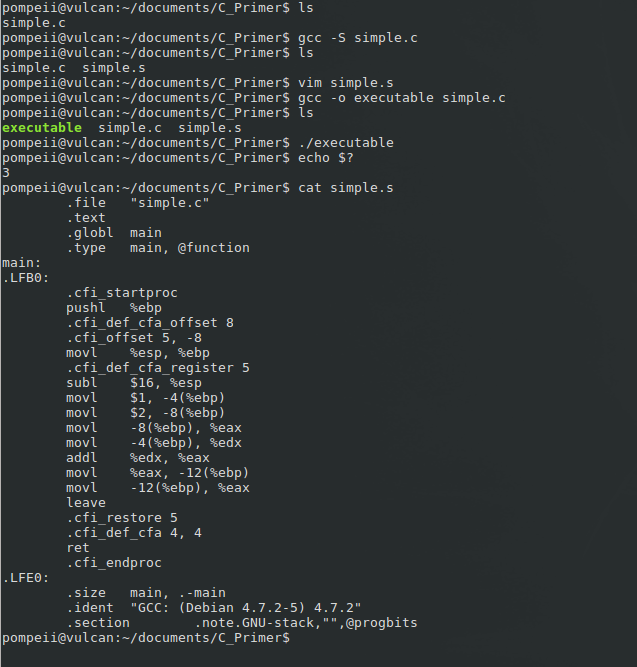
\includegraphics[width=\textwidth]{images/c_to_x86}}
\vskip 0.05in
\centerline{\textbf{Figure 2. }Simple C file compiled into x86}
\vskip 0.1in

The important portions to note in Figure 2 is the value returned by the function seen following the echo command (look for the '3') and the bottom half of the image in which the gcc generated assembly file is viewed. The GCC flag -S created the assembly file but did not generate the executable binaries. This program will not execute on its own. The -o flag following this created the executable that was subsequently run. The \textit{"ls"} commands list the files in the current directory in an Unix system. You can see the newly generated files following each GCC call.

\subsection{Programs}
One can see why C is considered such a strong low level language due to how thin the layer is between the program and ISA section. Unlike programs like Java or Python in which there are many additional layers of abstractions, C is translated directly into machine code. Starting at the other end of the levels of abstraction flow graph, we start off at the problem and algorithm stages. In terms of Robotathon this is where you will begin. Your end goal is to look at the overall problem, break the problem down into smaller modules and develop algorithms to solve them. Once you have an idea of how you can solve the problem in a step by step manner, you reach the program level. This is the level where the ambiguity of human language needs to be removed. At its core that is the purpose for programming languages. They give humans a way to translate our spoken language into a format that can control electrons all the way at the transistor level.

\section{Mechanics of C}
A C program consists of a set of sequentially executed instructions. Each line is terminated with a semi-colon to delimit the end of an instruction. These instructions will typically execute on data stored in variables. 

\subsection{Variables}
Variables are memory locations that are allocated as temporary storage space. C is very powerful in the sense that you execute very closely to the physical memory, which is why I try to emphasize some of that here. There are a variety of data types within C that you must use to define a variable. Some of the more common data types include:
\begin{itemize}
	\item char - character
	\item int - integer
	\item float - floating point
\end{itemize}

Characters variables means that a single byte of memory is allocated. Integer values depend on the architecture's word size. If your computer is a 64 bit machine, an integer variable allocates 64 bits. Likewise, a 32 bit architecture allocates 32 bits. Chars are typically used to represent ASCII encoded letters (although it is important to note that in memory it is still just a set of bits. This means depending on how you interpret the bits it can be a number as well), while integers are used to represent whole numbers. Floating point variables allow us to use decimal or fractional values. Many embedded systems do not have hardware support for floating point numbers making them very expensive to use as they require a lot of additional software math to do basic arithmetic (this is one of the nice things about the LM4F launchpads: they contain a hardware floating point unit). C, as well as many other languages, has the capability to bundle together a set of variables into a package. This package is called a \textit{structure} or struct. 
\begin{framed}
	\begin{lstlisting}[language=C++,
	                   directivestyle={\color{black}}
        	            emph={int,char,double,float,unsigned},
                	     emphstyle={\color{blue}}
                	    ]
	struct complex {
		int real;
		int imaginary;
	};
	...
	int main(void) {
		struct complex a;
		a.real = 1;
		a.imaginary = 2;
	}
	\end{lstlisting}
\end{framed}
\vskip 0.1in
\centerline{\textbf{Figure 3. }Example of a structure definition and creation}
\vskip 0.1in

A structure acts as a new data type in most cases as can be seen in Figure 3. A new variable \textit{'a'} is created of type struct complex. What this means is that in the above example, two sequential memory words will be allocated for each integer in the structure. These two variables are accessed with a "." as seen above followed by the name of the desired sub component. A nice feature in C is the ability to use \textit{"typedefs"} to relabel things. It can be a bit annoying to type out "struct complex variablename" each time. Following the structure, one can type "typedef struct complex complex". This will remap the type "struct complex" to the type "complex". The basic format of typedef is as follows: 
\centerline{\textbf{typedef} [original name] [new name mapping]} 
This line can actually be combined with the struct definition as seen below in Figure 4 by replacing the [original name] component with the actual struct definition.\\

\fbox{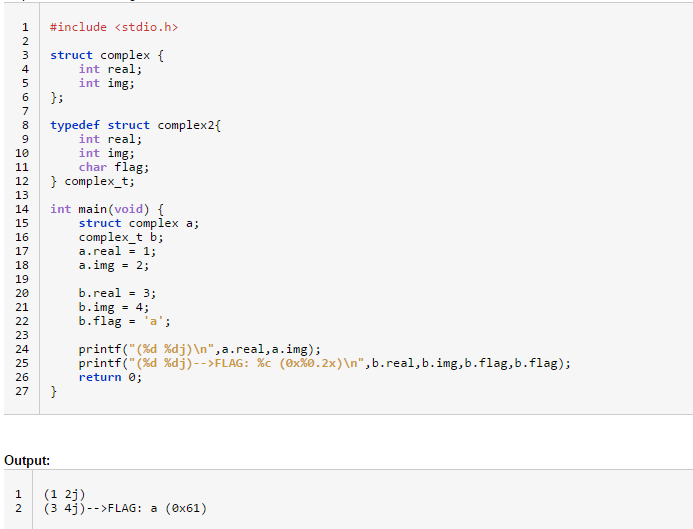
\includegraphics[width=\textwidth]{images/struct_sample}}
\vskip 0.05in
\centerline{\textbf{Figure 4. }Simple example of structures in C}
\vskip 0.1in

There is a lot of extra stuff in the image that we haven't really gotten to yet so I apologize for that. I will try my best to provide a step by step explanation of a sample file once I've covered the different structures within C.
\subsection{Flow of Execution}
While arithmetic and assignment operations are vital, we need to be able to actually control the flow of our program. This is done with three primary structures:
\begin{itemize}
	\item If-Statement - If a condition holds true, execute the following code segment. Can be followed by an \textit{else} block to create an if-else statement.
	\item While-Loop - While a condition holds true, execute the following code segment.
	\item For-Loop - Typically used for counting, execute the following code segment until the condition is no longer valid.
\end{itemize}

\newpage

\begin{framed}
	\begin{lstlisting}[language=C++,
	                   directivestyle={\color{black}}
        	            emph={int,char,double,float,unsigned},
                	     emphstyle={\color{blue}}
                	    ]
	while(x==1) {
		// do things while x is 1
	}
	...
	for(i=0; i<10; i=i+1) {
		// do things while i is less than 10.
		// increment i each iteration
	}
	...
	if(x==1) {
		// Execute this segment if x is 1.
	} else if(x==2) {
		// Execute this if x is 2 AND x is not 1.
	} else {
		// Execute this if x is not 1 or 2.
	}
	\end{lstlisting}
\end{framed}
\vskip 0.1in
\centerline{\textbf{Figure 5. }Example of a structure definition and creation}
\vskip 0.1in
\subsection{Functions}
Functions

\subsubsection{Input/Output (I/O)}
kbj

%%% End document
\end{document}
